\chapter{Empirical Evaluation} \label{ch:experiments}
This chapter presents the empirical results of all experimental configurations evaluated across the cohort of 36 patients. Section~\ref{sec:exp:baseline} establishes the baseline performance under standard MSE training. Sections~\ref{sec:exp:obj1} through~\ref{sec:exp:obj3} report the results for each of the three research objectives. Section~\ref{sec:exp:overall} provides a comprehensive comparative summary across all ten model configurations.

% ================================================================
\section{Baseline: Single-Step Forecasting} \label{sec:exp:baseline}
% ================================================================

Under standard MSE training, the T1DATA cohort results reproduce the systematic prediction delay described in Chapter~\ref{ch:introduction} and anticipated by preliminary PRG experiments~\citep{prg_glucose_proposal}. As established in Chapter~\ref{ch:introduction}, the strong lag-1 autocorrelation of the CGM signal (Section~\ref{sec:method:setup:cgm}) causes MSE training to reward reproducing recent glucose history: a prediction that mirrors the input window at a temporal offset incurs almost no gradient penalty, because consecutive glucose readings are nearly identical. The consequence, across both architectures, is a predicted trajectory that is structurally close to the true signal but displaced forward in time. The baseline established here therefore serves as the expected reference point for the ablation study: it instantiates the known failure mode under controlled conditions before any modification to the training objective is introduced.

Fig.~\ref{fig:exp:baseline_curves} illustrates this effect for a representative 10-hour segment. In both the LSTM (left) and PatchTST (right) panels, the predicted trajectory (blue dashed) follows the shape of the ground truth CGM signal (black solid) closely throughout the displayed window. The descent toward the 70~mg/dL hypoglycaemia threshold, however, occurs visibly later in the prediction than in the true signal, and the predicted trough is similarly displaced. The offset is not specific to the hypoglycaemic episode: it can be observed in both the rising and falling phases of the trajectory before and after the event, which suggests that it is a persistent property of the training objective rather than an isolated response to any particular glucose pattern.

\begin{figure}[tbp]
    \centering
    
\includegraphics[width=0.9\textwidth]{patient_85102.png}
    \caption[Baseline 60min prediction]{Baseline 60-minute forecasting trajectories for patient 85102 over a representative 10-hour window containing a hypoglycaemia episode. LSTM (left) and PatchTST (right) are shown side by side. The black line is the ground truth CGM signal; the blue dashed line is the model prediction. The red dashed line marks the 70~mg/dL hypoglycaemia threshold.}
    \label{fig:exp:baseline_curves}
\end{figure}

Tab.~\ref{tab:exp:baseline} quantifies what Fig.~\ref{fig:exp:baseline_curves} shows visually. Both architectures produce mean lags of approximately the full 60-minute forecast horizon, consistent with the autocorrelation argument above: rather than learning to anticipate future glucose behaviour, the model effectively reproduces the input window shifted forward in time. RMSE$^*$ separates the timing component from residual shape inaccuracy; the gap between RMSE and RMSE$^*$ shows that a substantial fraction of the raw prediction error is attributable purely to the temporal displacement and disappears once alignment is applied. Notably, this fraction is proportionally larger for PatchTST than for LSTM, despite the two architectures producing similar absolute lags, which suggests that PatchTST's raw error is more dominated by the timing offset than LSTM's.

Whether the delay visible in Fig.~\ref{fig:exp:baseline_curves} is representative of the full cohort can be assessed from Fig.~\ref{fig:exp:lag_dist}, which shows the per-patient distribution of $\Delta^*$ across all 36 patients for both architectures. Both distributions are compact and almost entirely positive: nearly all patients exhibit a delay in the same direction, with only a small number deviating substantially from the cohort median. The consistency in both direction and magnitude across patients supports the interpretation that the delay is a systematic consequence of the MSE objective applied to the highly autocorrelated signal, rather than a patient-specific artefact.

\begin{figure}[tbp]
    \centering
    
\includegraphics[width=0.55\textwidth]{lag_distribution.png}
    \caption{Boxplot of the per-patient prediction delay $\Delta^*$ for the LSTM and PatchTST baseline models. Each point represents one of the 36 patients. $\Delta^*$ is the temporal shift in minutes that minimises the per-patient RMSE between the shifted prediction and the ground truth.}
    \label{fig:exp:lag_dist}
\end{figure}

Tab.~\ref{tab:exp:baseline} reports the complete set of cohort-mean baseline metrics. The event detection columns, derived by thresholding the 60-minute prediction at 70~mg/dL with $\tau = 15$~minutes, reflect the direct clinical consequence of the timing offset: with the predicted trajectory displaced by approximately the full forecast horizon, the threshold crossing tends to arrive at or after the true hypoglycaemic onset rather than in advance of it. The two architectures also show notably different baseline detection behaviour—the LSTM triggers alarms at near-zero frequency, while PatchTST produces more alarms but at markedly low precision—and whether this divergence is driven by the MSE training objective or by architectural properties is a question examined in Section~\ref{sec:exp:obj3}.

\begin{table}[tbp]
\centering
\small
\caption{Baseline single-step forecasting performance under standard MSE training. RMSE$^*$ is the lag-adjusted RMSE after the optimal per-patient temporal shift $\Delta^*$. Mean Lag is the average absolute shift in minutes ($|\Delta^*| \times 5$~min). RMSE, RMSE$^*$, and MAE are in mg/dL; event-detection metrics are derived by thresholding the 60-min prediction at 70~mg/dL with $\tau = 15$~min. Means over 36 patients.}
\label{tab:exp:baseline}
\begin{tabular}{lrrrrrrrr}
\toprule
Model & RMSE & RMSE$^*$ & Lag (min) & MAE & Precision & Recall & F1 & F2 \\
\midrule
LSTM\,MSE      & 36.09 & 21.65 & 51.2 & 27.12 & 0.010 & 0.004 & 0.005 & 0.004 \\
PatchTST\,MSE  & 39.27 & 14.21 & 55.3 & 29.00 & 0.048 & 0.089 & 0.061 & 0.074 \\
\bottomrule
\end{tabular}
\end{table}

% ================================================================
\section{Objective 1: Offset-Aware Loss Functions} \label{sec:exp:obj1}
% ================================================================

This section addresses the first research question (Section~\ref{sec:method:obj1}): whether replacing MSE with an offset-aware loss function reduces the systematic prediction delay, and whether any such reduction improves event detection. The Bounded-Lag loss and Soft-DTW are assessed separately; a joint interpretation is provided at the end of this section.

\subsection{Bounded-Lag Loss Results}

The Bounded-Lag loss (Section~\ref{sec:bg:losses:bl}) forgives timing errors within a fixed local window of $D$ steps; the question here is whether this conservative relaxation is enough to move the predicted trajectory earlier in time.

Tab.~\ref{tab:exp:obj1} shows that the mean lag decreases for both architectures relative to the MSE baseline, but the reduction is small in relation to the baseline displacement documented in Section~\ref{sec:exp:baseline}: the residual delay remains close to the full 60-minute forecast horizon for both architectures, only a few minutes below the baseline values. RMSE and MAE change only marginally, indicating that the local tolerance window does not substantially reshape the predicted trajectory — it shifts its temporal position by a small amount without altering its overall form.

RMSE$^*$ reveals a further aspect of this pattern: despite the reduction in mean lag, the lag-adjusted error rises for both architectures relative to the MSE baseline. The lag decrease is therefore accompanied by a degradation of trajectory shape accuracy once the temporal offset is removed. Event detection shows a small improvement in F2 for both architectures, but the gain is modest relative to the detection failure documented in Section~\ref{sec:exp:baseline}. Notably, both architectures respond in the same direction under the Bounded-Lag loss — reduced lag, increased RMSE$^*$, marginal F2 gain — which suggests a consistent response pattern rather than architecture-specific behaviour.

\subsection{Soft-DTW Loss Results}

The Soft-DTW loss~\citep{cuturi2017softdtw} (Section~\ref{sec:bg:losses:sdtw}) takes a more aggressive approach to temporal tolerance than the Bounded-Lag loss by elastically warping the time axis to align the shapes of the predicted and true sequences. Rather than accepting matches within a fixed local window, it allows many-to-one correspondences across the full sequence, penalising shape mismatch instead of pointwise displacement at fixed time steps.

Fig.~\ref{fig:exp:obj1_predictions} shows the predicted trajectories for all three training strategies overlaid on the same representative window used in Section~\ref{sec:exp:baseline}. In the LSTM panel (left), the three curves diverge visibly around the descent toward the hypoglycaemia threshold: the Soft-DTW prediction arrives at the episode earlier than the MSE baseline, with the Bounded-Lag prediction lying between them. The overall shape of the predicted trajectory is preserved but its temporal position differs across strategies. In the PatchTST panel (right), the temporal separation between strategies is less pronounced, while the Soft-DTW prediction departs more noticeably from the ground truth in amplitude across the displayed window.

These visual differences are consistent with the quantitative pattern in Tab.~\ref{tab:exp:obj1}. For LSTM, Soft-DTW achieves the largest lag reduction of all evaluated configurations in this section, and RMSE remains within a few percent of the MSE baseline. The RMSE$^*$ column shows, however, that the lag-adjusted error rises further under Soft-DTW than under Bounded-Lag: the more aggressive temporal realignment degrades trajectory shape accuracy more, not less. Event detection does not improve in line with the lag reduction — F2 remains close to the MSE baseline and recall decreases slightly — suggesting that the temporal advance visible in Fig.~\ref{fig:exp:obj1_predictions} does not align the predicted threshold crossing more reliably with the true event.

For PatchTST, the response is markedly different in character. The lag reduction is substantially smaller than for LSTM — smaller even than that achieved by Bounded-Lag for LSTM — yet the RMSE increase is the largest observed across all configurations in Tab.~\ref{tab:exp:obj1}. RMSE$^*$ rises by a similarly large margin. The event detection figures show an increase in recall, but the precision column reveals a corresponding rise in false alarms, so the net effect on F2 is small. PatchTST thus incurs a large accuracy cost with minimal temporal gain, while LSTM achieves meaningful temporal advance at a moderate cost: the two architectures respond to the same loss in a qualitatively different way.

The Bounded-Lag loss produced no such asymmetry — both architectures showed qualitatively similar responses. That Soft-DTW breaks this symmetry suggests that it interacts differently with structural properties of the two architectures. What those properties are is a question the event-centric analysis in Section~\ref{sec:exp:obj3} and the overall comparison in Section~\ref{sec:exp:overall} will return to.

\begin{figure}[tbp]
    \centering
    
\includegraphics[width=\textwidth]{obj1_all_predictions.png}
    \caption{Prediction trajectories for all three Objective~1 training strategies on a representative patient window (patient 85102, 10-hour window containing a hypoglycaemia episode). LSTM (left) and PatchTST (right) are shown side by side; all three predictions are overlaid against the ground truth CGM signal. Line colours and styles distinguish the three training objectives as indicated in the legend.}
    \label{fig:exp:obj1_predictions}
\end{figure}

\begin{table}[tbp]
\centering
\small
\caption{Effect of offset-aware loss functions on forecasting accuracy and mean prediction delay. RMSE$^*$ is the lag-adjusted RMSE after the optimal per-patient temporal shift $\Delta^*$. Lag is the average absolute shift in minutes ($|\Delta^*| \times 5$~min). RMSE, RMSE$^*$, and MAE are in mg/dL; event-detection metrics are derived by thresholding each 60-min prediction at 70~mg/dL with $\tau = 15$~min. Bold values mark the best result per column across all configurations. Means over 36 patients.}
\label{tab:exp:obj1}
\resizebox{\textwidth}{!}{%
\begin{tabular}{llrrrrrrrr}
\toprule
Architecture & Loss & RMSE & RMSE$^*$ & Lag (min) & MAE & Precision & Recall & F1 & F2 \\
\midrule
\multicolumn{10}{l}{\textit{LSTM}} \\[2pt]
 & MSE (baseline) & \textbf{36.09} & 21.65          & 51.2          & \textbf{27.12} & 0.010 & 0.004 & 0.005 & 0.004 \\
 & Bounded-Lag    & 36.14          & 25.25          & 48.6          & 27.57          & 0.017 & 0.012 & 0.014 & 0.013 \\
 & Soft-DTW       & 37.23          & 28.67          & \textbf{46.0} & 28.76          & 0.039 & 0.009 & 0.014 & 0.010 \\
\midrule
\multicolumn{10}{l}{\textit{PatchTST}} \\[2pt]
 & MSE (baseline) & 39.27 & \textbf{14.21} & 55.3 & 29.00 & 0.048          & 0.089          & 0.061          & 0.074          \\
 & Bounded-Lag    & 39.30 & 16.70          & 54.6 & 29.03 & 0.055          & 0.095          & \textbf{0.066} & 0.080          \\
 & Soft-DTW       & 43.24 & 24.01          & 54.4 & 32.25 & \textbf{0.056} & \textbf{0.129} & 0.062          & \textbf{0.084} \\
\bottomrule
\end{tabular}}
\end{table}

Across both strategies, Tab.~\ref{tab:exp:obj1} reveals a consistent pattern: in every architecture-loss combination, RMSE$^*$ rises above the MSE baseline even as the mean lag falls. The offset-aware losses achieve a partial temporal realignment, but this comes at a cost to lag-adjusted trajectory accuracy that grows with the aggressiveness of the temporal tolerance. Neither strategy improves event detection to a degree that closes the gap observed at baseline. Whether this reflects a fundamental limitation of the optimisation approach — tolerating timing errors during training rather than removing the cause of the delay — or whether it depends on how each loss interacts with specific architectural properties, is a question the subsequent sections will address.

% ================================================================
\section{Objective 2: Multi-Step Forecasting} \label{sec:exp:obj2}
% ================================================================

Multi-step supervision~\citep{fox2018multioutput} addresses the second research question (Section~\ref{sec:method:obj2}): whether supervising the full forecast trajectory rather than a single endpoint reduces the prediction delay and improves event detection. The single output at $t+H$ is replaced by 12 simultaneous predictions at $t+1, \ldots, t+H$, with the MSE loss computed uniformly across all predicted steps. This is the only modification relative to the single-step baseline: architecture, hyperparameters, and all other training settings remain identical. Tab.~\ref{tab:exp:obj2} and Fig.~\ref{fig:exp:multistep_plot} report the results.

Fig.~\ref{fig:exp:multistep_plot} shows the predicted trajectories for both architectures overlaid against the ground truth on the same representative window used in Sections~\ref{sec:exp:baseline} and~\ref{sec:exp:obj1}. For LSTM (left panel), the multi-step prediction tracks the ground truth marginally more closely than the single-step baseline, particularly in the smoother portions of the trajectory before and after the hypoglycaemic episode. The temporal position of the threshold crossing, however, does not shift noticeably: the predicted curve still descends toward the hypoglycaemia threshold at a similar delay. For PatchTST (right panel), the two predictions are visually close throughout the displayed window, with small amplitude differences but no systematic temporal advance.

\begin{figure}[tbp]
    \centering
    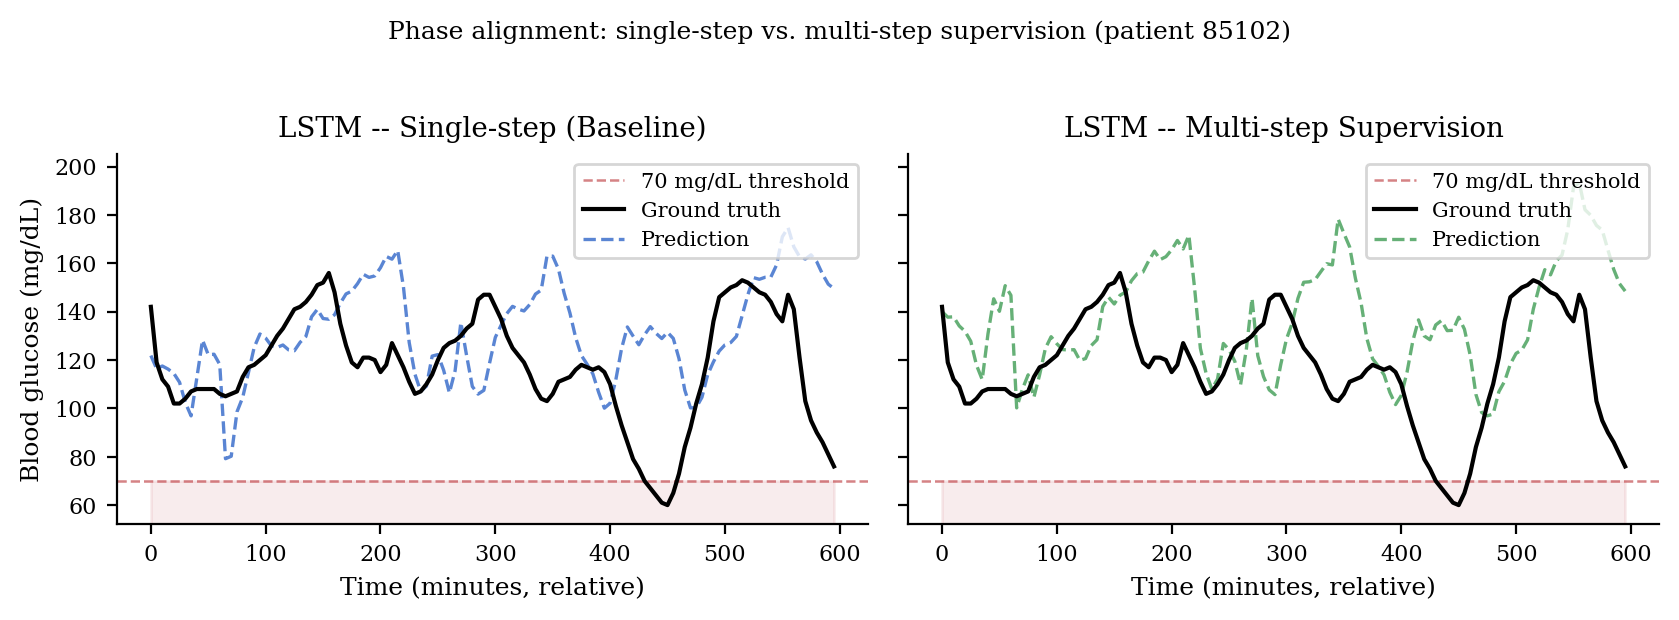
\includegraphics[width=\textwidth]{multistep_vs_baseline_trace.png}
    \caption{Prediction trajectories for LSTM (left) and PatchTST (right) on a representative patient window (patient 85102) containing a hypoglycaemia episode. The single-step baseline and multi-step predictions are overlaid against the ground truth CGM signal. Line colours and styles are as indicated in the legend.}
    \label{fig:exp:multistep_plot}
\end{figure}

Tab.~\ref{tab:exp:obj2} quantifies these observations. Multi-step supervision yields the best absolute RMSE and MAE of all configurations in this study for the LSTM, and the best RMSE and MAE among PatchTST variants. The improvement is consistent in direction across both architectures, though modest in magnitude; this confirms, in the CGM setting and for both architectures, the accuracy benefit of full-trajectory supervision reported by \citet{fox2018multioutput} and introduced in Chapter~\ref{ch:introduction}. The RMSE$^*$ column reveals an asymmetry: for LSTM, the lag-adjusted error decreases slightly under multi-step supervision, suggesting the broader training signal improves trajectory shape beyond what temporal alignment alone accounts for. For PatchTST, the relationship reverses — RMSE$^*$ increases marginally — indicating that the multi-step model trades a small amount of shape accuracy for the improvement visible in raw RMSE. The two architectures therefore respond in different ways to the same modification, a pattern that has also been observed in Section~\ref{sec:exp:obj1}.

The mean lag column shows that the temporal displacement of the predicted trajectory is nearly unchanged for both architectures. Broader supervision across all 12 output steps does not reduce the fundamental delay: the model produces more accurate values at individual steps but still exhibits the same overall temporal offset documented in Section~\ref{sec:exp:baseline}. This dissociation between improved point-wise accuracy and unchanged temporal structure is a key observation: it suggests that trajectory quality and temporal alignment are not tightly coupled, and that improving one does not automatically improve the other.

The event detection columns of Tab.~\ref{tab:exp:obj2} show a small increase in recall for both architectures under multi-step supervision, with precision changing little. F2 improves slightly in both cases. Whether this recall improvement reflects a genuine structural change in how the model anticipates threshold crossings, or whether it follows mechanically from the marginal improvement in trajectory accuracy, is a question the tolerance sweep in Section~\ref{sec:exp:obj3} will shed light on. More broadly, the finding that the configuration with the best trajectory accuracy does not produce the best event detection — and that the lag remains essentially unchanged despite the accuracy gains — raises a fundamental question about the relationship between forecasting quality and detection performance. This question is taken up in Section~\ref{sec:exp:overall}.

\begin{table}[tbp]
\centering
\small
\caption{Effect of multi-step sequence supervision on forecasting accuracy and mean prediction delay. RMSE$^*$ is the lag-adjusted RMSE after the optimal per-patient temporal shift $\Delta^*$. RMSE, RMSE$^*$, and MAE are in mg/dL; event-detection metrics are derived by thresholding each 60-min prediction at 70~mg/dL with $\tau = 15$~min. Bold values mark the best result per column across all configurations. Means over 36 patients.}
\label{tab:exp:obj2}
\resizebox{\textwidth}{!}{%
\begin{tabular}{llrrrrrrrr}
\toprule
Architecture & Supervision & RMSE & RMSE$^*$ & Lag (min) & MAE & Precision & Recall & F1 & F2 \\
\midrule
\multicolumn{10}{l}{\textit{LSTM}} \\[2pt]
 & Single-step (baseline) & 36.09 & 21.65          & 51.2          & 27.12 & 0.010 & 0.004 & 0.005 & 0.004 \\
 & Multi-step             & \textbf{35.59} & \textbf{20.74} & \textbf{50.1} & \textbf{26.80} & 0.011 & 0.009 & 0.010 & 0.010 \\
\midrule
\multicolumn{10}{l}{\textit{PatchTST}} \\[2pt]
 & Single-step (baseline) & 39.27 & \textbf{14.21} & 55.3 & 29.00 & 0.048 & 0.089          & 0.061          & 0.074          \\
 & Multi-step             & 39.05 & 14.53          & 54.6 & 28.84 & \textbf{0.060} & \textbf{0.103} & \textbf{0.072} & \textbf{0.085} \\
\bottomrule
\end{tabular}}
\end{table}

% ================================================================
\section{Objective 3: Event-Centric Evaluation} \label{sec:exp:obj3}
% ================================================================

This section addresses the third research question (Section~\ref{sec:method:obj3}): whether task-specific binary classifiers outperform threshold-based detection derived from regression forecasts. It evaluates hypoglycaemia detection from three complementary perspectives. The tolerance sweep quantifies how much of the detection failure of forecast-derived detectors is attributable to timing mismatch rather than a structural inability to produce threshold crossings. The direct classification analysis tests whether a task-specific training objective resolves the detection gap. The lead-time analysis examines how much advance warning the classifiers provide in practice.

\subsection{Forecast-Derived Detection: Tolerance Sweep}
\label{sec:exp:obj3:tausweep}

The tolerance sweep evaluates how forecast-derived event detection changes as the acceptance window $\tau$ is widened from 0 to 60~minutes in 5-minute steps (Section~\ref{sec:bg:metrics}). The key question it addresses is diagnostic: does detection fail because the model never predicts a threshold crossing, or because it predicts one at the wrong time? Full numerical results are provided in Tabs.~\ref{tab:app:tau_sweep_lstm} and~\ref{tab:app:tau_sweep_patchtst} in Appendix~\ref{appendix:detailed_metrics}.

For LSTM, Fig.~\ref{fig:exp:tau_sweep_lstm} shows the Precision, Recall, and F2 curves across the full $\tau$ range for all four training strategies evaluated in Sections~\ref{sec:exp:baseline} through~\ref{sec:exp:obj2}. The Recall panel shows a gradual increase as $\tau$ widens for all four strategies, but the absolute level remains modest throughout the range. The F2 curves follow the same pattern: a shallow, approximately linear rise without any steep inflection that would indicate a reservoir of temporally displaced detections being recovered. The Precision panel shows low values throughout; for several strategies, precision decreases as $\tau$ widens, as the broader acceptance window admits increasing numbers of predicted crossings that do not correspond to true events.

The four strategies overlap closely across all three panels. The Soft-DTW LSTM achieved the largest mean lag reduction of all configurations (Section~\ref{sec:exp:obj1}), yet its F2 curve does not rise above the MSE baseline. The Multi-step LSTM produced the best absolute trajectory accuracy (Section~\ref{sec:exp:obj2}) but also shows no distinctive advantage across the sweep. Neither lag reduction nor improved trajectory fidelity produces a curve that diverges meaningfully from the others. The near-uniform behaviour across strategies, combined with the shallow rise in recall, is consistent with a model that produces few predicted threshold crossings regardless of how wide the timing tolerance becomes — rather than one whose detections are structurally present but systematically displaced.

\begin{figure}[tbp]
    \centering
    
\includegraphics[width=\textwidth]{tau_sweep_appendix_lstm.png}
    \caption{Cohort-mean Precision, Recall, and F2 as a function of the tolerance window $\tau$ for all four LSTM training strategies (MSE, Bounded-Lag, Soft-DTW, Multi-step). Each panel shows one metric; line colours and styles correspond to the training objective as indicated in the legend. Detailed numerical values are in Tab.~\ref{tab:app:tau_sweep_lstm}.}
    \label{fig:exp:tau_sweep_lstm}
\end{figure}

The PatchTST tau sweep, shown in Fig.~\ref{fig:exp:tau_sweep_patchtst}, presents a different picture. Beginning from the same fixed-$\tau$ starting points reported in Sections~\ref{sec:exp:baseline} through~\ref{sec:exp:obj2}, the F2 curves rise steeply and reach substantially higher values as $\tau$ widens toward 60~minutes. The Recall panel shows a rapid increase across the full range for all four strategies, reaching high values at the widest window — a gain that is qualitatively distinct from anything observed in the LSTM sweep. The steep recall rise suggests that predicted threshold crossings exist in the PatchTST output in the vicinity of true hypoglycaemic events, but fall outside the narrow acceptance window used in the fixed-$\tau$ evaluation of the preceding sections.

The Precision panel for PatchTST tells a more cautious story. Values remain moderate and decline as $\tau$ widens, because the broader window also admits more false alarms alongside the recovered true positives. F2 rises because the recall gain is large enough to dominate despite this precision cost — a direct consequence of the F2 weighting scheme defined in Section~\ref{sec:bg:metrics}. The trade-off between recall and precision, and how it evolves with $\tau$, is visible in the diverging trajectories of the two panels.

Comparing the four training strategies in Fig.~\ref{fig:exp:tau_sweep_patchtst}, the curves cluster closely throughout the full $\tau$ range. The Soft-DTW PatchTST incurred the largest RMSE increase of all configurations (Section~\ref{sec:exp:obj1}) yet its sweep curve is indistinguishable from the MSE baseline. The Multi-step PatchTST produced the best PatchTST trajectory accuracy (Section~\ref{sec:exp:obj2}) and shows at most a marginal separation at wider $\tau$ values. Neither modifying the loss for temporal tolerance nor extending the supervision horizon produces a systematic shift in when PatchTST crosses the threshold.

\begin{figure}[tbp]
    \centering
    
\includegraphics[width=\textwidth]{tau_sweep_appendix_patchtst.png}
    \caption{Cohort-mean Precision, Recall, and F2 as a function of the tolerance window $\tau$ for all four PatchTST training strategies (MSE, Bounded-Lag, Soft-DTW, Multi-step). Each panel shows one metric; line colours and styles correspond to the training objective as indicated in the legend. Detailed numerical values are in Tab.~\ref{tab:app:tau_sweep_patchtst}.}
    \label{fig:exp:tau_sweep_patchtst}
\end{figure}

The contrast between Figs.~\ref{fig:exp:tau_sweep_lstm} and~\ref{fig:exp:tau_sweep_patchtst} is the central finding of this section. For LSTM, widening the acceptance window yields only marginal improvement across all training strategies, suggesting that the detection gap may not be closeable by relaxing timing constraints alone. For PatchTST, widening the window recovers a large fraction of detections, suggesting that predicted threshold crossings exist in the output but fall outside the narrow fixed-$\tau$ window. Whether this points to a timing displacement that a different training objective could correct, or to a deeper structural difference between the two architectures, is a question Section~\ref{sec:exp:obj3:classifiers} begins to address by comparing forecast-derived performance against directly trained binary classifiers.

\subsection{Direct Binary Event Classifiers}
\label{sec:exp:obj3:classifiers}

Direct binary classifiers~\citep{shao2024hypoglycemia, cinar2025hypoclassification} are trained end-to-end on the event label defined in Equation~\ref{eq:eventlabel}, using a weighted binary cross-entropy loss to address the class imbalance (Section~\ref{sec:method:setup:cgm}). Unlike the forecast-derived detectors evaluated in the preceding sections, these classifiers optimise directly for the binary detection objective rather than applying a threshold to a regression output.

Tab.~\ref{tab:exp:classifiers} reports the cohort-mean performance of both classifiers. Both architectures achieve considerably higher recall than the best forecast-derived detector for their respective architecture, as documented in Sections~\ref{sec:exp:obj1} through~\ref{sec:exp:obj3:tausweep}. The gains in F2 over the best forecast-derived baselines are considerable for both architectures and hold for the large majority of individual patients, as the per-patient F2 standard deviations reported in Tab.~\ref{tab:exp:classifiers} reflect.

\begin{table}[tbp]
\centering
\small
\caption{Direct binary event classifier performance on the 60-minute hypoglycaemia prediction horizon. F2 weights recall twice as heavily as precision, reflecting the asymmetric cost of missed events relative to false alarms as defined in Section~\ref{sec:bg:metrics}. Bold values mark the best result per column. Means over 36 patients; F2 standard deviations: LSTM~0.175, PatchTST~0.137.}
\label{tab:exp:classifiers}
\begin{tabular}{lrrrr}
\toprule
Model & Precision & Recall & F1 & F2 \\
\midrule
LSTM event classifier     & \textbf{0.237} & \textbf{0.693} & \textbf{0.334} & \textbf{0.463} \\
PatchTST event classifier & 0.054          & 0.615          & 0.095          & 0.178          \\
\bottomrule
\end{tabular}
\end{table}

A notable feature of Tab.~\ref{tab:exp:classifiers} is the pronounced asymmetry in the precision column between the two classifiers. The LSTM classifier achieves a considerably higher precision alongside its recall, while the PatchTST classifier registers markedly lower precision despite achieving comparable recall. The F2 scores of the two architectures therefore reflect different precision-recall profiles: the LSTM achieves high recall at moderate precision, whereas PatchTST achieves similar recall at considerably lower precision. The per-patient variability is also notable: the F2 standard deviations indicate that both classifiers vary considerably across the cohort.

A second observation from Tab.~\ref{tab:exp:classifiers} concerns the performance ordering between architectures. In all forecasting tasks evaluated in Sections~\ref{sec:exp:baseline} through~\ref{sec:exp:obj2}, the LSTM consistently achieves lower RMSE than PatchTST. In the classification task, this ordering reverses: the LSTM event classifier achieves a considerably higher F2 than the PatchTST classifier, with the gap visible across all four metrics in the table. The performance ranking thus depends on the task objective, and the architecture that is the more accurate forecaster is not the more accurate event detector.


The precision difference between the two classifiers is made visible in Fig.~\ref{fig:exp:classifier_traces}, which shows the predicted event probability over time for a representative patient segment. In the LSTM panel (top), the probability trace rises selectively in the vicinity of the shaded true-positive regions, with extended periods of low predicted probability between events. In the PatchTST panel (bottom), the probability trace remains elevated more broadly across the displayed segment, including during periods that fall outside the true-positive regions. This pattern is consistent with the low precision value in Tab.~\ref{tab:exp:classifiers}: a large proportion of PatchTST alarms fall outside labelled hypoglycaemic windows. What drives this difference in alarm selectivity between the two architectures is a question that Section~\ref{sec:exp:overall} and Chapter~\ref{ch:conclusions} will address.

\begin{figure}[tbp]
    \centering
    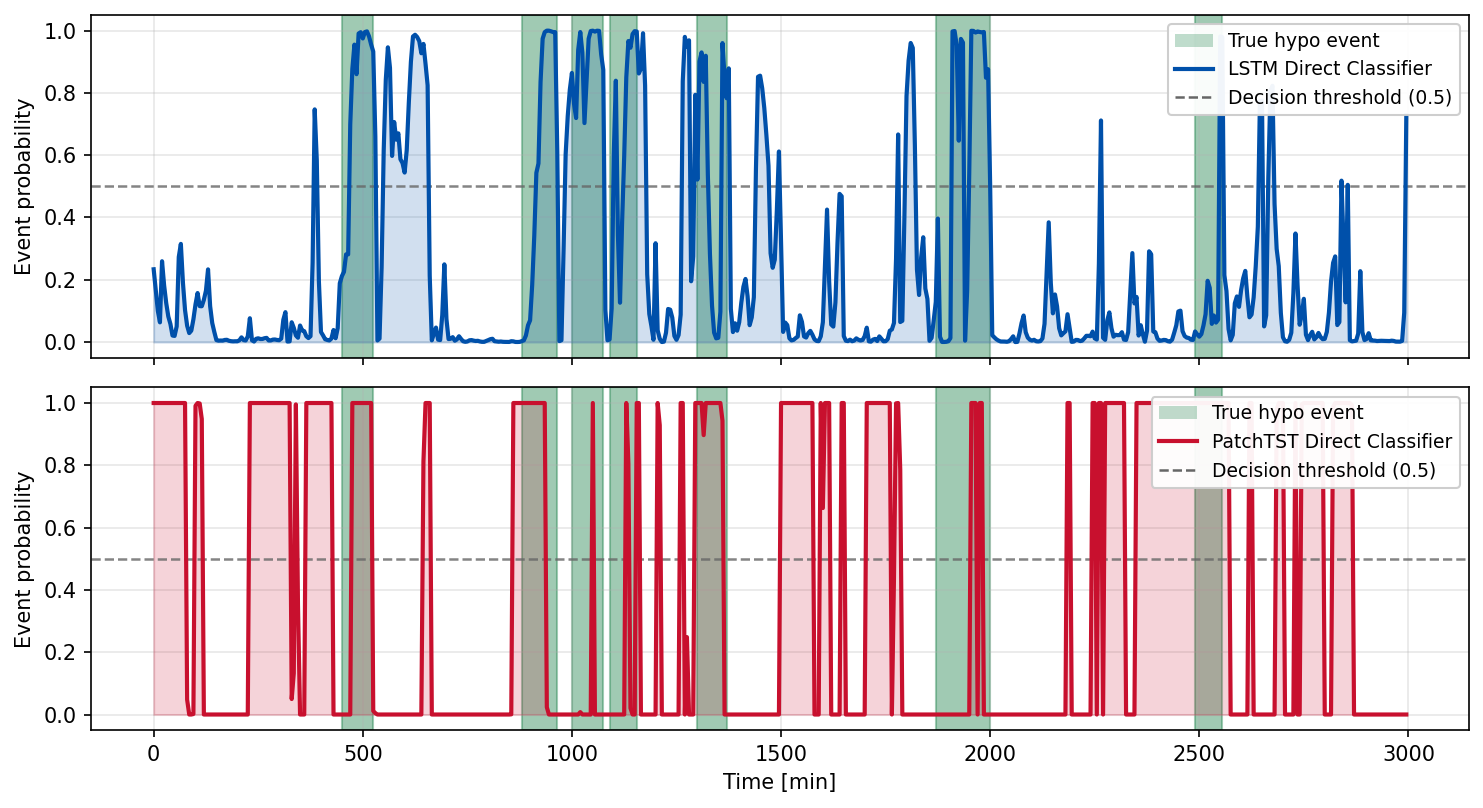
\includegraphics[width=0.9\textwidth]{classifier_predictions.png}
    \caption{Output traces of the LSTM (top) and PatchTST (bottom) direct event classifiers for a representative patient segment. The predicted event probability is plotted against time; the shaded regions indicate windows where the ground truth label is positive. The absolute confusion counts across the full cohort are shown in Fig.~\ref{fig:app:confusion_counts}.}
    \label{fig:exp:classifier_traces}
\end{figure}

Beyond the aggregate metrics and the alarm distribution visible in Fig.~\ref{fig:exp:classifier_traces}, a further dimension of the detection results concerns the timing of true-positive alarms relative to the hypoglycaemic event. The F2 metric counts an alarm as correct if it fires within the 60-minute prediction horizon, but does not distinguish between an alarm issued well in advance of the event and one issued at the moment the patient has already entered the hypoglycaemic range. This distinction is the focus of Section~\ref{sec:exp:obj3:leadtime}.

\subsection{Lead-Time Analysis}
\label{sec:exp:obj3:leadtime}

The transition from Section~\ref{sec:exp:obj3:classifiers} identified a dimension of detection performance that the F2 metric does not capture: whether a true-positive alarm fires before the hypoglycaemic event or at the moment it has already begun. The lead-time analysis quantifies this directly. Lead time is defined as the elapsed time from alarm issuance to the first hypoglycaemic step in the prediction window; a value of zero minutes means the alarm fires when the patient has already crossed the 70~mg/dL threshold, while a positive value indicates the alarm precedes the event.

Fig.~\ref{fig:exp:lead_time} shows the cohort-level distribution of lead times for all true-positive detections of both classifiers, binned at 5-minute intervals. The two distributions have markedly different shapes. For the LSTM classifier, the zero-lead-time bar is the tallest by a considerable margin: alarms that fire at event onset represent the largest single group of true positives, after which the distribution drops sharply and spreads across the remaining bins. For the PatchTST classifier, the zero-lead-time bar is smaller relative to the total, and the remaining bins are populated more evenly across the 5-to-55 minute range.

\begin{figure}[tbp]
    \centering
    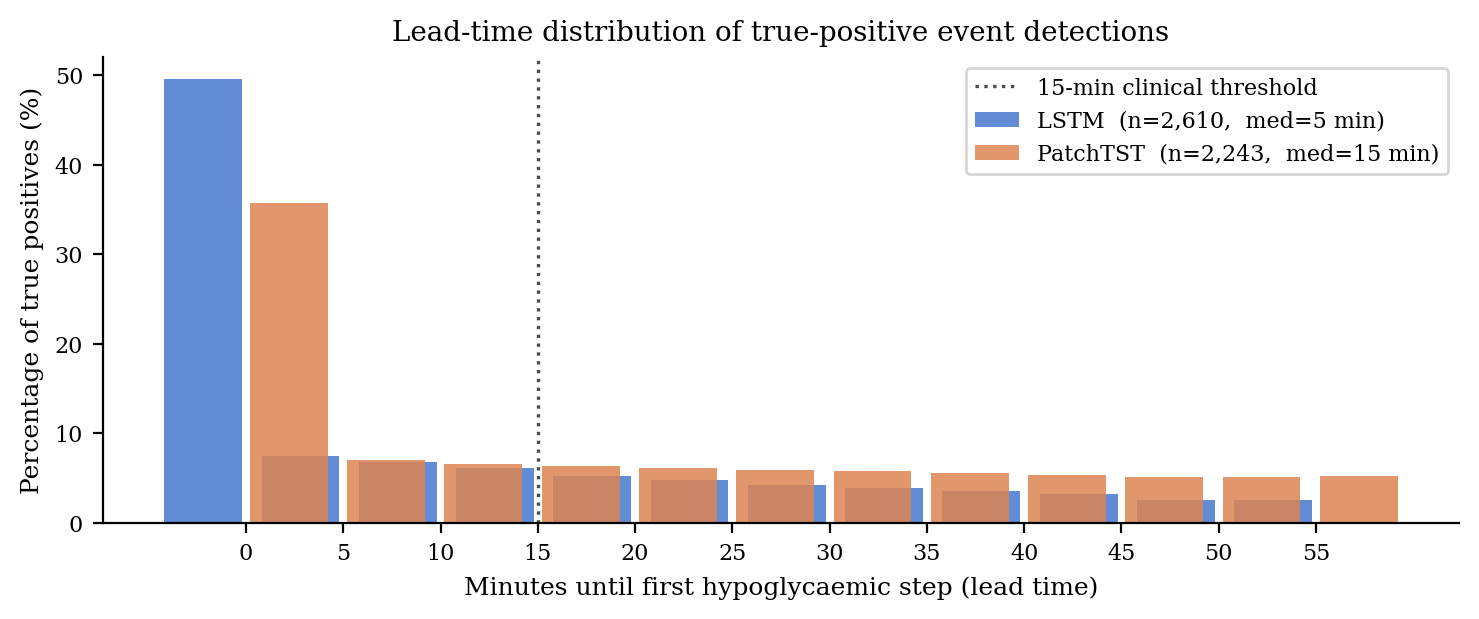
\includegraphics[width=0.9\textwidth]{lead_time_distribution.png}
    \caption{Distribution of lead times for true-positive detections by the LSTM and PatchTST direct event classifiers across the 36-patient cohort. Lead time is the elapsed time in minutes from alarm issuance to the first hypoglycaemic step in the prediction window. Bars are grouped by model and binned at 5-minute intervals; the median lead time per model is shown in the legend.}
    \label{fig:exp:lead_time}
\end{figure}

The numbers behind Fig.~\ref{fig:exp:lead_time} quantify the contrast. Of the LSTM's 2{,}610 true positives across the cohort, 1{,}293 — close to half — fire at lead time zero, yielding a median of 5~minutes and a mean of 12.4~minutes. Of the PatchTST's 2{,}243 true positives, 802 (35.8\%) fall at zero lead time; the remainder are distributed across the 5-to-55 minute range, producing a median of 15~minutes and a mean of 18.3~minutes. Despite achieving lower overall recall, the PatchTST classifier issues a larger proportion of its true-positive alarms before the patient enters the hypoglycaemic range.

The two classifiers therefore exhibit different alarm-timing profiles. The LSTM distribution — dominated by the zero-lead-time bin — is consistent with a classifier that responds primarily when glucose values are at or near the threshold at alarm time; the broadcast alarm density visible in Fig.~\ref{fig:exp:classifier_traces} reinforces this picture. The PatchTST distribution — flatter and shifted toward positive lead times — suggests that its alarms are triggered more frequently by glucose patterns that precede the crossing, even if the lower total true-positive count reflects its lower recall. The difference in these profiles adds a dimension to the classifier comparison that the aggregate F2 values in Tab.~\ref{tab:exp:classifiers} do not convey on their own.

Considering that a preventive response to an anticipated hypoglycaemic episode may itself require a window of time — as the pharmacodynamic delays described in Chapter~\ref{ch:introduction} suggest — the timing of true-positive alarms relative to event onset is a relevant property of a detection system alongside its recall. How the two dimensions of detection performance and anticipatory profile should be weighted, and what the observed distributions imply for the practical utility of each classifier, is discussed in Chapter~\ref{ch:conclusions}.


% ================================================================
\section{Overall Comparison} \label{sec:exp:overall}
% ================================================================

Across the ten configurations evaluated in Sections~\ref{sec:exp:baseline} through~\ref{sec:exp:obj3:leadtime}, no single configuration leads on both trajectory quality and event detection performance. This section draws together the patterns that run across the individual sections — not to restate what each section reported, but to make visible the structural relationships between those findings that the subsequent conclusions will build on.

\paragraph{Trajectory metrics and temporal displacement respond independently to training changes.}
A consistent pattern across Objective~1 is that every configuration that reduces the mean lag also increases RMSE$^*$: partial temporal realignment comes at a cost to trajectory shape accuracy, and the two metrics move in opposite directions. Objective~2 adds a complementary observation: multi-step supervision achieves the best absolute trajectory accuracy of any configuration without reducing the lag meaningfully. Together, these findings show that RMSE, lag, and RMSE$^*$ can be moved independently by training changes — and that improving one does not automatically improve the others.

\paragraph{The best trajectory configuration and the best detection configuration do not coincide.}
The configuration that leads on RMSE and MAE (LSTM multi-step) is not the one that leads on event detection F2 (LSTM direct classifier). Among the forecast-derived configurations, improving trajectory accuracy does not translate into event detection gains of comparable magnitude: the F2 scores of all eight forecast-derived configurations remain in a narrow band, well below the direct classifiers. The tau sweep in Objective~3 provides the diagnostic explanation for part of this gap: the LSTM rarely produces predicted threshold crossings regardless of timing tolerance, while PatchTST produces many but displaced in time. The two architectures therefore face structurally different obstacles to event detection under forecast-derived evaluation.

\paragraph{The two architectures diverge consistently across all three objectives.}
The performance difference between LSTM and PatchTST is not confined to a single evaluation context: it appears in the asymmetric RMSE response to Soft-DTW in Objective~1, in the opposite RMSE$^*$ trends under multi-step supervision in Objective~2, in the qualitatively different tau sweep curves in Objective~3, and in the performance inversion between forecasting and classification tasks. This recurrent divergence suggests that the two architectures differ in how they represent glucose trajectories near the hypoglycaemia threshold — a structural difference that the aggregate metrics alone do not fully characterise.

\paragraph{Direct classification changes the detection picture, but adds a new dimension.}
The direct classifiers achieve considerably higher recall than any forecast-derived configuration, establishing that end-to-end training on the event label addresses the detection gap that all forecasting-based approaches leave open. However, the lead-time analysis in Section~\ref{sec:exp:obj3:leadtime} reveals that detection performance and anticipatory capability are not the same property: the two classifiers occupy different positions in a two-dimensional space defined by these two dimensions, and F2 alone captures only one of them. Which dimension is more important, and what the observed distributions imply for the practical utility of each classifier, are questions that depend on how the system is intended to be used.

These four patterns — the independent behaviour of trajectory and lag metrics, the disconnect between trajectory quality and detection performance, the architectural divergence, and the two-dimensionality of classifier evaluation — define what the experimental results collectively establish. Chapter~\ref{ch:conclusions} draws the conclusions that follow from them.

